%______________________________________________________
%
%   LaTeX-mall fr nybrjare
%
%   Konstruerad av Marcus Bergner, bergner@cs.umu.se
%
%   Vid funderingar titta lngst ned i denna fil,
%   eller skicka ett mail
%______________________________________________________
%

% lite instllningar
\documentclass[10pt, titlepage, oneside, a4paper]{article}
\usepackage[T1]{fontenc}
\usepackage[utf8]{inputenc}
\usepackage[swedish]{babel}
\usepackage{amssymb, graphicx, fancyheadings}
\usepackage{placeins}
\addtolength{\textheight}{20mm}
\addtolength{\voffset}{-5mm}
\renewcommand{\sectionmark}[1]{\markleft{#1}}

% \Section ger mindre spillutrymme, anvnd dem om du vill
\newcommand{\Section}[1]{\section{#1}\vspace{-8pt}}
\newcommand{\Subsection}[1]{\vspace{-4pt}\subsection{#1}\vspace{-8pt}}
\newcommand{\Subsubsection}[1]{\vspace{-4pt}\subsubsection{#1}\vspace{-8pt}}
	
% appendices, \appitem och \appsubitem r fr bilagor
\newcounter{appendixpage}

\newenvironment{appendices}{
	\setcounter{appendixpage}{\arabic{page}}
	\stepcounter{appendixpage}
}{
}

\newcommand{\appitem}[2]{
	\stepcounter{section}
	\addtocontents{toc}{\protect\contentsline{section}{\numberline{\Alph{section}}#1}{\arabic{appendixpage}}}
	\addtocounter{appendixpage}{#2}
}

\newcommand{\appsubitem}[2]{
	\stepcounter{subsection}
	\addtocontents{toc}{\protect\contentsline{subsection}{\numberline{\Alph{section}.\arabic{subsection}}#1}{\arabic{appendixpage}}}
	\addtocounter{appendixpage}{#2}
}

% ndra de rader som behver ndras
\def\inst{Institutionen för datavetenskap}
\def\typeofdoc{Labbrapport}
\def\course{Systemnära programmering 7.5hp}
\def\pretitle{Laboration 5}
\def\title{mfind\_p}
\def\name{Robin Lundberg}
\def\username{ens10rlg}
\def\email{\username{}@cs.umu.se}
\def\path{/home/rolund03/workspace/gsl_ode}
\def\graders{Mikael Rännar, Ola Ringdahl}


% om du vill referera till katalogen dr dina filer ligger kan du 
% anvnda \fullpath som kommer att vara "~username/edu..." o.s.v.
%\def\fullpath{\raisebox{1pt}{$\scriptstyle \sim$}\username/\path}


% Hr brjar sjlva dokumentet
\begin{document}

	% skapar framsidan (om den inte duger: gr helt enkelt en egen)
	\begin{titlepage}
		\thispagestyle{empty}
		\begin{large}
			\begin{tabular}{@{}p{\textwidth}@{}}
				\textbf{UMEÅ UNIVERSITET \hfill \today} \\
				\textbf{\inst} \\
				\textbf{\typeofdoc} \\
			\end{tabular}
		\end{large}
		\vspace{10mm}
		\begin{center}
			\LARGE{\pretitle} \\
			\huge{\textbf{\course}}\\
			\vspace{10mm}
			\LARGE{\title} \\
			\vspace{15mm}
			\begin{large}
				\begin{tabular}{ll}
					\textbf{Namn} & \name \\
					\textbf{E-mail} & \texttt{\email} \\
					\textbf{Sökväg} & \texttt{/home/ens10/ens10rlg/edu/sysprog/lab5} \\
				\end{tabular}
			\end{large}
			\vfill
			\large{\textbf{Handledare}}\\
			\mbox{\large{\graders}}
		\end{center}
	\end{titlepage}


	% fixar sidfot
	\lfoot{\footnotesize{\name, \email}}
	\rfoot{\footnotesize{\today}}
	\lhead{\sc\footnotesize\title}
	\rhead{\nouppercase{\sc\footnotesize\leftmark}}
	\pagestyle{fancy}
	\renewcommand{\headrulewidth}{0.2pt}
	\renewcommand{\footrulewidth}{0.2pt}

	% skapar innehllsfrteckning.
	% Tnk p att kra latex 2ggr fr att uppdatera allt
	\pagenumbering{roman}
	\tableofcontents
	
	% och lägger in en sidbrytning
	\newpage

	\pagenumbering{arabic}

	% i Sverige har vi normalt inget indrag vid nytt stycke
	\setlength{\parindent}{0pt}
	% men dremot lite mellanrum
	\setlength{\parskip}{10pt}

	% lägger in rubrik (finns \section, men då får man mycket spillutrymme)
	\FloatBarrier
	\Section{Problemspecifikation}
	
%Sökprogram som använder trådar, snabbare än program som inte använder trådar
Jag har implementerat en trådad sökalgoritm som ska kunna söker efter filer på hårddisken rekursivt ner i
mappstrukturer. Målet är att programmet ska vara snabbare för datorer med flera kärnor än vad ett otrådad
program som utför samma uppgift är. Detta kräver att trådarna belastas ungefär lika.

%mfind_p [-t type] [-p nrthr] start1 [start2 ...] name
Programmet körs med kommandot \texttt{mfind\_p [-t type] [-p nrthr] start1 [start2 ...] name}.
\texttt{mfind\_p} är programmet; \texttt{startx} är mappar som man ska börja söka rekursivt i;
\texttt{name} är namnet på den fil man ska söka efter; \texttt{type} specifierar vilken typ av fil du 
vill hitta, man kan välja mellan d, f och l som innebär mapp, vanlig fil eller mjuk länk respektive; \texttt{nrthr} anger hur många trådar man vill använda för att köra programmet.

%Pool of tasks
För att genomföra denna sökning ska varje tråd ges en mapp---från en \emph{taskpool} som enabrt den får söka i---tråden ska sedan fylla på denna taskpool med mappar som den hittar i denna mapp; sedan ska den också leta efter det \emph{namn} som användaren vill söka efter och sedan skriva ut den. Detta sker i en loop tills alla undermappar har sökts igenom.

%Synkronisering. Deadlock, pool of tasks, inga task, avslut.
För att undvika \emph{deadlock} och \emph{odefinierade beteenden} när trådarna utnyttjar gemensamt minne så måste trådarna synkroniseras. Trådarna måste även kunna hantera en tillfälligt tom taskpool och veta när dom kan avsluta.



	\FloatBarrier
	\Section{Åtkomst och användarhandledning}
	%1. How to compile the program
To compile the disassembler, run \texttt{make dismips}.
%2. How to run the program
Run the disassembler by executing the command \texttt{dismips file}.
Where \texttt{file} is the path to the file containing the MIPS32 machine code to be disassembled.
The disassembler supports all instructions except those with op-code 16, 17 and 18 except for the commands
\texttt{bclf}, \texttt{bclt}, \texttt{mfc1} and \texttt{mtc1} which are included.

%3. How is the output formatted
The disassembler outputs to \emph{standard out} the following for each line of machine code:
\begin{enumerate}
\item the original instruction.
\item the type of instruction.
\item the values for relevant fields for that type of instruction in decimal.
\item the values for relevant fields for that type of instruction in hexadecimal.
\item and the mnemonic representation.
\end{enumerate}
in the format \texttt{1; 2; 3; 4; 5;} where the numbers corresponds to the information in the list above.
The disassembler will output error messages that corresponds to whatever type of error is in the machine code e.g. if you try to use a floating point instruction it will tell you it is not allowed or if you use an invalid op- or function-code it will also tell you that---and then continue with the next line of machine code.		

	\FloatBarrier
	\Section{Algoritmbeskrivning}
	Main programmet kommer sköta initialisering av variabler, mutex och tolkningen av inargument.
Sedan så skapar huvudtråden N-1 trådar som kör funktionen \texttt{taskManager} som i sin tur kallar på \texttt{mfind\_p}. Huvudtråden kommer sedan själv köra taskManager och när alla trådar är färdiga så städar huvudtråden upp efter processen.
Det behövs fyra globala variabler för att sköta synkningen mellan trådarna och dom är:
\texttt{waiting} som anger hur många trådar som inte kör \texttt{mfind\_p}, utan väntar på att en task ska läggas till i taskpoolen; \texttt{blocked} som är en array där varje element anger huruvida den motsvarande tråd väntar på en task eller inte, detta är för att förhindra att en tråd ökar på \texttt{waiting} flera gånger då tråden inte kommer sluta loopa bara för att den inte har någon task; \texttt{quit} som signalerar till trådarna att nu kan dom avsluta funktionen för sökningen är färdig, detta kommer ske när \texttt{waiting} är lika med antalet trådar; och till sist en \texttt{taskpool} som innehåller relativa sökvägar till dom mappar som behövs gås igenom.

%TODO: Beskriv dom mutexar som används
\def\accessTaskPoolMutex{accessTaskPool}
\def\getTaskMutex{getTask}
\def\initThreadIDMutex{initThreadID}
Programmet använder tre mutexar för att hantera synkroniseringen mellan trådar.
\texttt{\initThreadIDMutex} används för att ge varje tråd ett unikt id mellan 0 och $N-1$ om $N$ är antalet trådar.
\texttt{\accessTaskPoolMutex} används för att förhindra att olika trådar försöker komma åt \texttt{taskpoolen} samtidigt vilket kan ge odefinierat beteende.
\texttt{\getTaskMutex} används för att kunna bestämma när trådarna kan avsluta.

\Subsection{taskManager}
\begin{enumerate}
\item \texttt{count = 0}
\item	Ge tråden ett unikt \texttt{id}.
\item	Kör loop tills färdig.
	\begin{enumerate}
	\item	Lås \getTaskMutex.
		\begin{enumerate}
		\item	Lås \accessTaskPoolMutex.
			\begin{enumerate}
			\item	\texttt{mapp = getFolderFromTaskPool()}
			\end{enumerate}
		\item	Lås upp \accessTaskPoolMutex.
		\item 	Om \texttt{mapp == NULL} och om \texttt{!blocked[id]}. Öka då på \texttt{waiting} med ett och sätt \texttt{blocked[id] == true}.
		\item	Om \texttt{mapp != NULL} så sätt \texttt{waiting = 0} till 0 och alla element i \texttt{blocked} till \texttt{false}.
		\item 	Om \texttt{waiting == N} så sätt \texttt{quit} till \texttt{true}
		\end{enumerate}
	\item	Lås upp \getTaskMutex.
	\item	Om \texttt{mapp == NULL} och \texttt{quit == true}
		\begin{enumerate}
		\item	Gå ut ur loopen.
		\end{enumerate}
	\item	Om \texttt{mapp == NULL} och \texttt{quit == false}
		\begin{enumerate}
		\item	Börja om loopen.
		\end{enumerate}
	\item	Om \texttt{mapp != NULL}
		\begin{enumerate}
		\item	Kör \texttt{mfind\_p} med \texttt{mapp} som inargument.
		\item	Öka på \texttt{count} med ett.
		\end{enumerate}	
	\end{enumerate}
\item	Skriv ut tråd-id och \texttt{count}.
\item	Avsluta funktionen.
\end{enumerate}


\Subsection{mfind\_p}
Funktionen \texttt{mfind\_p} har som argument en sökväg till en mapp och två variabler som används för att
bestämma om en fil är den man söker efter.
\begin{enumerate}
\item	Öppna \texttt{mapp} på given sökväg.
\item 	Gå igenom alla filer i mappen.
	\begin{enumerate}
	\item	Kolla om filen är den du söker efter. Skriv i så fall ut dess sökväg på standard output.
	\item 	Om filen är en mapp och inte "." eller "..", gör följande
		\begin{enumerate}
		\item	Lås \accessTaskPoolMutex
			\begin{enumerate}
			\item	Lägg till ny mapp i \texttt{taskpool}
			\end{enumerate}
		\item	Lås upp \accessTaskPoolMutex	
		\end{enumerate}
	\end{enumerate}
\item	Stäng mappen.
\item 	Avsluta funktionen.
\end{enumerate}

	
	\FloatBarrier
	\Section{Systembeskrivning}
	\Subsection{Datastrukturer}

\Subsubsection{node}
En länkad lista används för att implementera en stack. I det här programmet behövs en stack för att
spara dom mappar som programmet ska söka i, kallad \texttt{taskpool}.

\Subsection{Viktiga variabler}

\Subsection{Funktioner}
\Subsubsection{int main(int argc, char *argv[])}
Läser in argument och initialiserar mutexar och variabler. Huvudtråden ser till att de andra trådarna
kör \texttt{taskManager}. Huvudtråden kör sedan också \texttt{taskManager}. När alla trådar är klar med \texttt{taskManager} så städar huvudtråden upp och programmet avslutas.

\Subsubsection{void * taskManager(void *pArg)}
Hanterar synkroniseringen mellan trådarna. Det som i slutändan görs är att kalla \texttt{mfind\_p}
tills alla mappar som ska sökas igenom; har blivit genomsökta.

\Subsubsection{void mfind\_p(char *path, pcre *find, int type)}
Kollar upp alla filer i gen givna mappen på \texttt{path}. Ifall filen är den som söks---d.v.s. den är av typen \texttt{type} och passar det reguljära uttrycket \texttt{find}---så skrivs sökvägen
ut på standard output. Ifall filen är en mapp men inte "." eller ".." så sparas den i stacken (\texttt{taskpoolen}) för att någon tråd ska kunna använda den som argument i \texttt{mfind\_p}. 

\Subsubsection{void read\_arguments(int argc, char *argv[], par\_t *par)}
Tolkar inargument och verifierar att dom är på rätt format.

\Subsubsection{char * popTask(void)}
Tar bort den mapp som ligger högst upp i stacken från stacken(\texttt{taskpoolen}) och returnerar den.

\Subsubsection{void pushTask(char* v)}
Lägger till en mapp till stacken (\texttt{taskpoolen}).

\Subsection{Anropsdiagram}
\begin{figure}[h!]
	\centering
	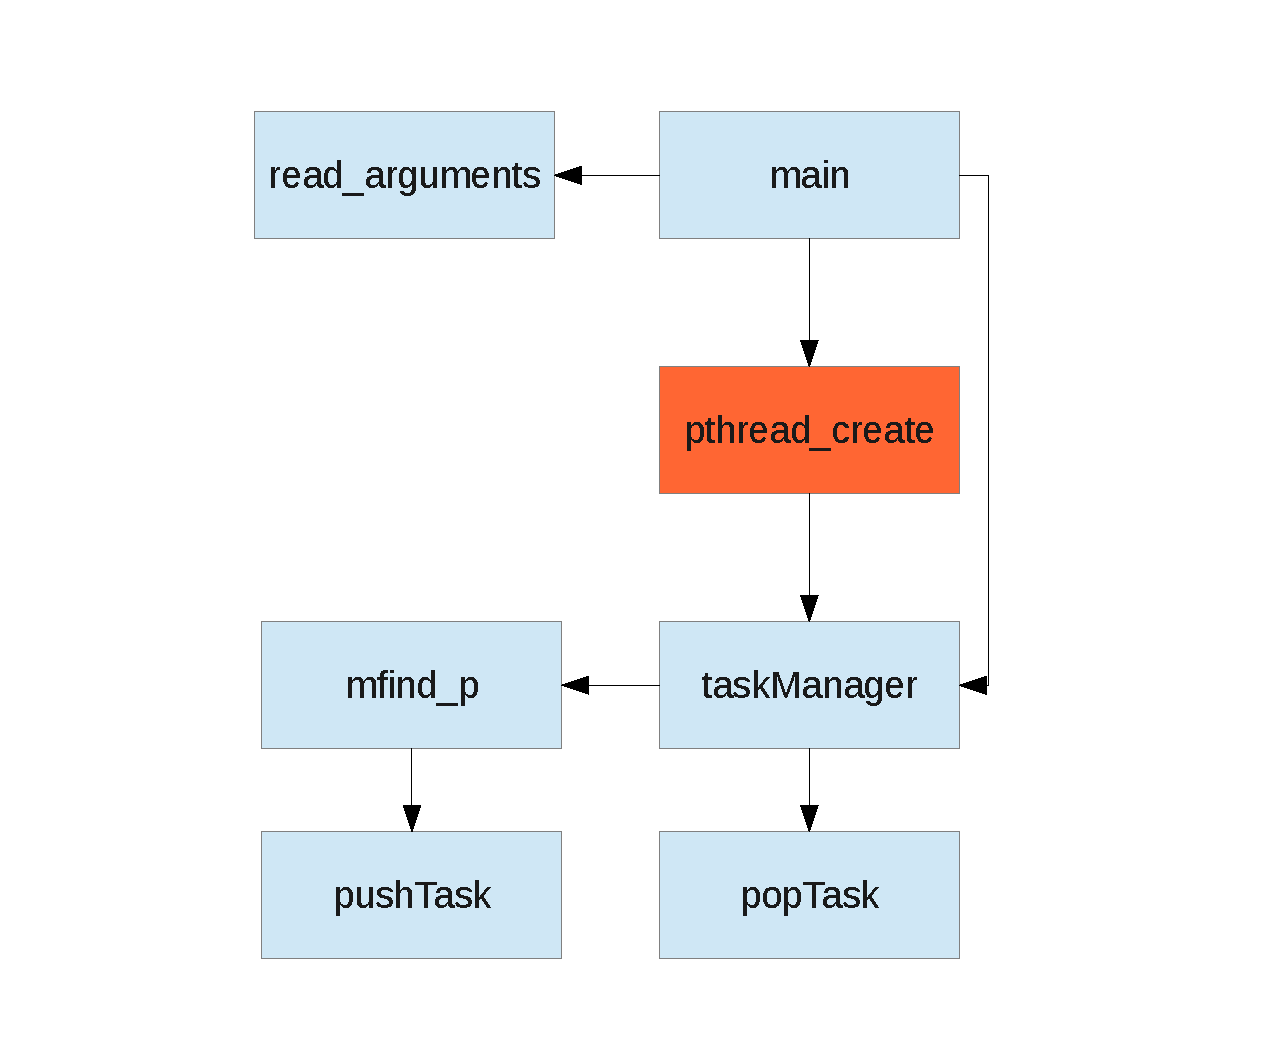
\includegraphics[width=0.8\textwidth]{img/anropsdiagram}
	\caption{Anropsdiagram för programmet mfind\_p.}
	\label{fig:anropsdiagram}
\end{figure}


	\FloatBarrier
	\Section{Testkörningar}
	För att testa programmet har en känd mappstruktur skapats med följande skript.
\begin{verbatim}
#!/bin/sh
mkdir newtest
ln -s newtest linktest
cd newtest
mkdir a
ln -s a b
cd a
mkdir b c d
ln -s b a
cd b
mkdir a b c
chmod 000 c
touch d
cd a
touch a
cd ..
touch b/a b/c
\end{verbatim}

Resultaten ska bli,  och blir följande:
\begin{verbatim}
%./mfind_p -p2 newtest b
newtest/b
newtest/a/b
newtest/a/b/b
No permission to open newtest/a/b/c
140329278105344: 4
140329288730368: 4

%./mfind_p -p2 -t l newtest b
newtest/b
No permission to open newtest/a/b/c
139734134916864: 3
139734124291840: 5

%./mfind_p -p2 -t d newtest linktest b
newtest/a/b
linktest/a/b
linktest/a/b/b
No permission to open linktest/a/b/c
newtest/a/b/b
No permission to open newtest/a/b/c
140144795088640: 9
140144805713664: 7
\end{verbatim}

	\FloatBarrier
	\Section{Begränsningar}
	Man kan inte ange hur djup man vill söka i mappstrukturen. Programmet kollar inte om antalet trådar som användaren anger är ett korrekt nummer. Det finns inget som begränsar användaren att ange samma startmapp mer än en gång. 

	\FloatBarrier
	\Section{Problem och reflektioner}
	Det var väldigt svårt att få till synkronisering mellan trådar så att dom avslutar när dom är färdig;
det tog mer tid än allt annat. Från början hade jag tänkt använda mig av semaforer men så vitt jag vet inte fanns inte så kallade \emph{counting semaphores} implementerade, dvs. semaforerna kunde inte räkna upp till mer än ett. Vilket är ett problem om du exempelvis vill utnyttja dom för att hålla koll på antalet tasks som finns i taskpoolen; det jag istället gjorde var att använda mutexar och globala variabler.
	
		

%	% här brjar alla bilagor. Denna måste finnas med även om bara
%	% bilagor anges i \begin{appendices} ... \end{appendices}
%	\appendix
%
%	\Section{Bilaga 1}
%	\ldots{}ligger direkt i dokumentet
%
%	% bilagor, t.ex. källkod. En tom extrasida kommer att skrivas ut för
%	% att få alla sidnummer att stämma
%	\begin{appendices}
%		\appitem{Källkod}{0}
%		\appsubitem{\texttt{mish.c}}{2}
%		\appsubitem{\texttt{mish.h}}{1}
%		\appitem{En bilaga på 3 sidor}{3}
%	\end{appendices}

\end{document}


% Lite information om hur man arbetar med LaTeX
%-----------------------------------------------
%
% LaTeX-koden kan skrivas med en godtycklig editor.
% Fr att "kompilera" dokumentet anvnds kommandot latex:
%    bergner@peppar:~/edu/sysprog/lab1> latex rapportmall.tex
% Resultatet blir ett antal filer, bl.a. en som heter rapportmall.dvi.
% Denna fil kan anvndas fr att titta hur dokumentet egentligen ser
% ut med hjlp av programmet xdvi:
%    bergner@peppar:~/edu/sysprog/lab1> xdvi rapportmall.dvi &
% Du fr d upp ett fnster som visar ditt dokument. Detta fnster
% kommer automatiskt att uppdateras d du ndrar och kompilerar om din
% LaTeX-kod. 
% Nr du anser att din rapport r frdig att skrivas ut anvnder man
% lmpligtvis kommandona dvips och lpr:
%    bergner@peppar:~/edu/sysprog/lab1> dvips -P ma436ps rapportmall.dvi
% Om man vill ha kvar PostScript-filen som dvips genererar kan man gra:
%    bergner@peppar:~/edu/sysprog/lab1> dvips -o rapport.ps rapportmall.dvi
%    bergner@peppar:~/edu/sysprog/lab1> lpr -P ma436ps rapport.ps
% OBS!!! Fr att innehllsfrteckningen och eventuella referenser till
% tabeller och figurer garanterat ska stmma mste man kra latex 2ggr
% p sitt dokument efter att man har ndrat ngot.
%
%
% Lite information om saker man kan tnkas behva i sitt arbete med LaTeX
%-------------------------------------------------------------------------
%
% FORMATTERA TEXT
%
% Fr att formattera text p lite olika stt kan man anvnda fljande LaTeX-
% kommandon:
%    \textbf{denna text kommer att vara i fetstil}
%    \emph{denna text r viktig (kursiv stil)}
%    \texttt{i denna text blir alla tecken lika breda, som med en skrivmaskin}
%    \textsf{denna text visas med ett typsnitt utan serifer}
%
%
% MATEMATISKA FORMLER
%
% Fr att typstta matematiska formler kan man anvnda:
%    $f(x) = x^2 - 3$, vilket lgger in formeln i texten, eller
%    \begin{displaymath}
%        g(x) = \frac{\sin x}{x}
%    \end{displaymath}, vilket lter formeln visas centrerat p en egen rad
% Om du vill att en formel ska numreras byter du ut displaymath mot equation.
% Det finns massor med matematiska symboler, vilket gr att man behver
% ngon liten manual att titta i om man ska konstruera avancerade formler.
% Se slutet p filen fr lite rd om var du kan hitta sdana.
%
%
% INFOGA FIGURER
%
% Fr att infoga en figur kan man gra p fljande stt:
%    \begin{figure}[htb]
%        \includegraphics[scale=0.5, angle=90]{exec_flow.eps}
%        \caption{Detta r bildtexten}
%        \label{EXECFLOW}
%    \end{figure}
% Om man vill referera till denna bild i texten skulle man d skriva enligt:
%    ...i figur \ref{EXECFLOW} kan man se att...
% Ngra sm frklaringar till figurer:
%    [htb] = talar om hur latex ska frska placera bilden (Here, Top, Bottom)
%            Om du anvnder [!h], innebr det Here!!!
%    scale = kan skala om bilden, om den r skalbar
%    angle = kan rotera bilden
%    exec_flow.eps = filnamnet p bilden. Notera att formatet .EPS anvnds
% Fr att skapa figurer anvnds lmpligtvis programmet xfig:
%    bergner@peppar:~/edu/sysprog/lab1> xfig &
% Rita (och spara ofta) tills du r klar. Vlj sedan "Export" och exportera
% din figur till EPS-format.
% Om man vill kan man anvnda endast \includegraphics, men det r inte ofta
% man gr det.
%
%
% INFOGA TABELLER
%
% Om man vill skapa en tabell gr man p fljande stt:
%    \begin{table}[htb]
%        \begin{tabular}{|rlp{10cm}|}
%            \hline
%            13 & $17.26$ & En kommentar som kan strcka sig ver flera rader \\
%            \hline
%        \end{tabular}
%        \caption{Tabelltexten...}
%        \label{TBL:MINTABELL}
%    \end{table}
% Om man vill kan man endast anvnda raderna 2-6, dvs f en tabell utan text
% och nummer. Om man gr p detta vis kommer tabellen alltid att lggas p
% det stlle den skrivs i koden, dvs ungefr samma sak som [!h] -> Here!!!
% Ngra frklaringar:
%    l, r, c = vnsterjustera, hgerjustera eller centrera kolumn
%    p{bredd} = skapa en vnsterjusterad kolumn med en viss bredd
%               kan innehlla flera rader text
%    | = en vertikal linje i tabellen
%    \hline = en horisontell linje i tabellen
%    & = kolumnseparator
%    \\ = radseparator
% Tnk p att tabeller oftast ser bttre ut med ganska f linjer.
%
%
% INFOGA KLLKOD ELLER UTDATA FRN TESTKRNINGAR
%
% Om man vill infoga kllkod eller ngot annat liknande, t.ex. utdata frn
% en testkrning r det bra om LaTeX terger utdatan korrekt, dvs en radbrytning
% betyder en radbrytning och 8 mellanslag p rad betyder 8 mellanslag p rad.
% Fr att stadkomma detta anvnds:
%    \begin{verbatim}
%        allt som skrivs hr terges exakt, med skrivmaskinstypsnitt
%    \end{verbatim}
% Oftast finns det dock bttre verktyg fr att skriva ut kllkod. Exempel p
% sdana r a2ps, enscript och atp.
%
%
% NDRA STORLEK P TEXT
%
% Om du vill ndra storleken p ett stycke, t.ex. p din nyss infogade
% testkrning omger du stycket med \begin{STORLEK} \end{STORLEK}, dr
% STORLEK r ngon av:
%    tiny, scriptsize, footnotesize, small, normalsize, large, Large,
%    LARGE, huge, Huge
% Tnk p att inte mixtra fr mycket med storlekar bara.
%
%
% SKAPA LISTOR AV OLIKA SLAG
%
% Det r ganska vanligt att man vill rada upp saker p ngot stt. Fr att
% skapa punktlistor anvnds:
%    \begin{itemize}
%        \item Detta r frsta punkten
%        \item Detta r andra punkten
%    \end{itemize}
% Om man istllet vill ha en numrerad lista kan man anvnda enumerate istllet
% fr itemize. Listor kan anvndas i flera niver
%
%
% MER INFORMATION OM LaTeX
%
% Lite blandad information om LaTeX, lnkar och annat hittar du p
% http://www.cs.umu.se/~bergner/latex.htm
% En del information om rapportskrivning hittar du p
% http://www.cs.umu.se/~bergner/rapport/
% Det finns massor med information om LaTeX p Internet. Ett litet urval:
% http://www.giss.nasa.gov/latex/
%     r en mycket vlfylld sida om LaTeX
% http://wwwinfo.cern.ch/asdoc/WWW/essential/essential.html
%     r en manual som genererats utifrn ett LaTeX-dokument mha latex2html
% http://tex.loria.fr/english/
%     r ett fylligt arkiv av lnkar till LaTeX-dokument p Internet
%
% Min personliga favorit r dock manualen "The Not So Short Introduction to
% LaTeX2e", som finns i DVI-format p ~bergner/LaTeX/lshort2e.dvi
% Dr str i princip allt man behver veta. Det r bara att anvnda xdvi och
% titta efter det du sker, vilket oftast finns dr.
% Om du, precis som jag, vill kunna leka med mnga kommandon i LaTeX finns en
% "LaTeX Command Summary" p ~bergner/LaTeX/latexcmds.ps
